% Options for packages loaded elsewhere
\PassOptionsToPackage{unicode}{hyperref}
\PassOptionsToPackage{hyphens}{url}
%
\documentclass[
]{article}
\usepackage{amsmath,amssymb}
\usepackage{lmodern}
\usepackage{ifxetex,ifluatex}
\ifnum 0\ifxetex 1\fi\ifluatex 1\fi=0 % if pdftex
  \usepackage[T1]{fontenc}
  \usepackage[utf8]{inputenc}
  \usepackage{textcomp} % provide euro and other symbols
\else % if luatex or xetex
  \usepackage{unicode-math}
  \defaultfontfeatures{Scale=MatchLowercase}
  \defaultfontfeatures[\rmfamily]{Ligatures=TeX,Scale=1}
\fi
% Use upquote if available, for straight quotes in verbatim environments
\IfFileExists{upquote.sty}{\usepackage{upquote}}{}
\IfFileExists{microtype.sty}{% use microtype if available
  \usepackage[]{microtype}
  \UseMicrotypeSet[protrusion]{basicmath} % disable protrusion for tt fonts
}{}
\makeatletter
\@ifundefined{KOMAClassName}{% if non-KOMA class
  \IfFileExists{parskip.sty}{%
    \usepackage{parskip}
  }{% else
    \setlength{\parindent}{0pt}
    \setlength{\parskip}{6pt plus 2pt minus 1pt}}
}{% if KOMA class
  \KOMAoptions{parskip=half}}
\makeatother
\usepackage{xcolor}
\IfFileExists{xurl.sty}{\usepackage{xurl}}{} % add URL line breaks if available
\IfFileExists{bookmark.sty}{\usepackage{bookmark}}{\usepackage{hyperref}}
\hypersetup{
  pdftitle={Multiple flow FeNO in population research: R code methods demo},
  hidelinks,
  pdfcreator={LaTeX via pandoc}}
\urlstyle{same} % disable monospaced font for URLs
\usepackage[margin=1in]{geometry}
\usepackage{color}
\usepackage{fancyvrb}
\newcommand{\VerbBar}{|}
\newcommand{\VERB}{\Verb[commandchars=\\\{\}]}
\DefineVerbatimEnvironment{Highlighting}{Verbatim}{commandchars=\\\{\}}
% Add ',fontsize=\small' for more characters per line
\usepackage{framed}
\definecolor{shadecolor}{RGB}{248,248,248}
\newenvironment{Shaded}{\begin{snugshade}}{\end{snugshade}}
\newcommand{\AlertTok}[1]{\textcolor[rgb]{0.94,0.16,0.16}{#1}}
\newcommand{\AnnotationTok}[1]{\textcolor[rgb]{0.56,0.35,0.01}{\textbf{\textit{#1}}}}
\newcommand{\AttributeTok}[1]{\textcolor[rgb]{0.77,0.63,0.00}{#1}}
\newcommand{\BaseNTok}[1]{\textcolor[rgb]{0.00,0.00,0.81}{#1}}
\newcommand{\BuiltInTok}[1]{#1}
\newcommand{\CharTok}[1]{\textcolor[rgb]{0.31,0.60,0.02}{#1}}
\newcommand{\CommentTok}[1]{\textcolor[rgb]{0.56,0.35,0.01}{\textit{#1}}}
\newcommand{\CommentVarTok}[1]{\textcolor[rgb]{0.56,0.35,0.01}{\textbf{\textit{#1}}}}
\newcommand{\ConstantTok}[1]{\textcolor[rgb]{0.00,0.00,0.00}{#1}}
\newcommand{\ControlFlowTok}[1]{\textcolor[rgb]{0.13,0.29,0.53}{\textbf{#1}}}
\newcommand{\DataTypeTok}[1]{\textcolor[rgb]{0.13,0.29,0.53}{#1}}
\newcommand{\DecValTok}[1]{\textcolor[rgb]{0.00,0.00,0.81}{#1}}
\newcommand{\DocumentationTok}[1]{\textcolor[rgb]{0.56,0.35,0.01}{\textbf{\textit{#1}}}}
\newcommand{\ErrorTok}[1]{\textcolor[rgb]{0.64,0.00,0.00}{\textbf{#1}}}
\newcommand{\ExtensionTok}[1]{#1}
\newcommand{\FloatTok}[1]{\textcolor[rgb]{0.00,0.00,0.81}{#1}}
\newcommand{\FunctionTok}[1]{\textcolor[rgb]{0.00,0.00,0.00}{#1}}
\newcommand{\ImportTok}[1]{#1}
\newcommand{\InformationTok}[1]{\textcolor[rgb]{0.56,0.35,0.01}{\textbf{\textit{#1}}}}
\newcommand{\KeywordTok}[1]{\textcolor[rgb]{0.13,0.29,0.53}{\textbf{#1}}}
\newcommand{\NormalTok}[1]{#1}
\newcommand{\OperatorTok}[1]{\textcolor[rgb]{0.81,0.36,0.00}{\textbf{#1}}}
\newcommand{\OtherTok}[1]{\textcolor[rgb]{0.56,0.35,0.01}{#1}}
\newcommand{\PreprocessorTok}[1]{\textcolor[rgb]{0.56,0.35,0.01}{\textit{#1}}}
\newcommand{\RegionMarkerTok}[1]{#1}
\newcommand{\SpecialCharTok}[1]{\textcolor[rgb]{0.00,0.00,0.00}{#1}}
\newcommand{\SpecialStringTok}[1]{\textcolor[rgb]{0.31,0.60,0.02}{#1}}
\newcommand{\StringTok}[1]{\textcolor[rgb]{0.31,0.60,0.02}{#1}}
\newcommand{\VariableTok}[1]{\textcolor[rgb]{0.00,0.00,0.00}{#1}}
\newcommand{\VerbatimStringTok}[1]{\textcolor[rgb]{0.31,0.60,0.02}{#1}}
\newcommand{\WarningTok}[1]{\textcolor[rgb]{0.56,0.35,0.01}{\textbf{\textit{#1}}}}
\usepackage{graphicx}
\makeatletter
\def\maxwidth{\ifdim\Gin@nat@width>\linewidth\linewidth\else\Gin@nat@width\fi}
\def\maxheight{\ifdim\Gin@nat@height>\textheight\textheight\else\Gin@nat@height\fi}
\makeatother
% Scale images if necessary, so that they will not overflow the page
% margins by default, and it is still possible to overwrite the defaults
% using explicit options in \includegraphics[width, height, ...]{}
\setkeys{Gin}{width=\maxwidth,height=\maxheight,keepaspectratio}
% Set default figure placement to htbp
\makeatletter
\def\fps@figure{htbp}
\makeatother
\setlength{\emergencystretch}{3em} % prevent overfull lines
\providecommand{\tightlist}{%
  \setlength{\itemsep}{0pt}\setlength{\parskip}{0pt}}
\setcounter{secnumdepth}{-\maxdimen} % remove section numbering
\ifluatex
  \usepackage{selnolig}  % disable illegal ligatures
\fi

\title{Multiple flow FeNO in population research: R code methods demo}
\author{}
\date{\vspace{-2.5em}}

\begin{document}
\maketitle

The following demo file provides example R code to implement six methods
for research involving multiple flow exhaled nitric oxide (FeNO)
measurements in a study population, where the goal is to relate
estimated NO parameters to factors of interest (i.e., covariate(s) X).

\hypertarget{preliminaries-set-up-your-r-session}{%
\subsection{0. Preliminaries: set up your R
session}\label{preliminaries-set-up-your-r-session}}

IMPORTANT! Install JAGS, if not already installed, follow instructions
at: \url{https://mcmc-jags.sourceforge.io/}

Load the following required packages, installing first if not already
available. To use the R2jags package, JAGS must be pre-installed.

\begin{Shaded}
\begin{Highlighting}[]
\CommentTok{\# set working directory}
\FunctionTok{setwd}\NormalTok{(}\StringTok{"K:/paper/newpackage/PopFeNO"}\NormalTok{)}
\CommentTok{\# load required packages}
\FunctionTok{require}\NormalTok{(MASS)}
\FunctionTok{require}\NormalTok{(lme4)}
\FunctionTok{require}\NormalTok{(nlme)}
\FunctionTok{require}\NormalTok{(reshape2)}
\FunctionTok{require}\NormalTok{(R2jags)}
\end{Highlighting}
\end{Shaded}

\hypertarget{data-simulation}{%
\subsection{1. Data simulation}\label{data-simulation}}

First, set a random seed for your work.

\begin{Shaded}
\begin{Highlighting}[]
\FunctionTok{set.seed}\NormalTok{(}\DecValTok{2022}\NormalTok{)}
\end{Highlighting}
\end{Shaded}

Simulate data from a cross-sectional study with multiple flow FeNO and a
single standard normal covariate X using the function DataGeneratorCS()
in DataG.R, which outputs a simulated dataset for Ndat participants,
with data for each participant on mean flow and FeNO for all maneuvers
as well as that participant's value of X.

\begin{Shaded}
\begin{Highlighting}[]
\CommentTok{\# Simulate a multiple flow FeNO dataset in a study population}
\FunctionTok{source}\NormalTok{(}\StringTok{"DataG.R"}\NormalTok{)       }\CommentTok{\# code to generate multiple flow FeNO datasets}
\NormalTok{flow}\OtherTok{=}\FunctionTok{c}\NormalTok{(}\FunctionTok{rep}\NormalTok{(}\DecValTok{30}\NormalTok{,}\DecValTok{2}\NormalTok{),}\FunctionTok{rep}\NormalTok{(}\DecValTok{50}\NormalTok{,}\DecValTok{2}\NormalTok{),}\FunctionTok{rep}\NormalTok{(}\DecValTok{100}\NormalTok{,}\DecValTok{2}\NormalTok{),}\FunctionTok{rep}\NormalTok{(}\DecValTok{300}\NormalTok{,}\DecValTok{2}\NormalTok{))}
\NormalTok{truebeta}\OtherTok{=}\FunctionTok{c}\NormalTok{(}\FloatTok{0.1}\NormalTok{,}\FloatTok{0.1}\NormalTok{,}\FloatTok{0.1}\NormalTok{)}
\NormalTok{out }\OtherTok{\textless{}{-}} \FunctionTok{DataGeneratorCS}\NormalTok{(}\AttributeTok{Ndat=}\DecValTok{500}\NormalTok{,           }\CommentTok{\# number of study participants}
                      \AttributeTok{alpha=}\FunctionTok{c}\NormalTok{(}\FloatTok{1.5}\NormalTok{,}\FloatTok{3.5}\NormalTok{,}\FloatTok{2.5}\NormalTok{),}\CommentTok{\# vector of NO parameter population means, }
                                           \CommentTok{\# when X=0, in this order: CA, logCaw, logDaw}
                      \AttributeTok{Xfn=}\ControlFlowTok{function}\NormalTok{(n)\{}\FunctionTok{rnorm}\NormalTok{(n,}\DecValTok{0}\NormalTok{,}\DecValTok{1}\NormalTok{)\}, }\CommentTok{\# function to generate participant{-}level covariate X }
                                                     \CommentTok{\# as function of number of study participants}
                      \AttributeTok{beta=}\NormalTok{truebeta, }\CommentTok{\# vector of regression coefficients relating X to NO parameters, }
                                           \CommentTok{\# in this order: CA, logCaw, logDaw}
                      \AttributeTok{Flow=}\FunctionTok{c}\NormalTok{(}\FunctionTok{rep}\NormalTok{(}\DecValTok{30}\NormalTok{,}\DecValTok{2}\NormalTok{),}\FunctionTok{rep}\NormalTok{(}\DecValTok{50}\NormalTok{,}\DecValTok{2}\NormalTok{),}\FunctionTok{rep}\NormalTok{(}\DecValTok{100}\NormalTok{,}\DecValTok{2}\NormalTok{),}\FunctionTok{rep}\NormalTok{(}\DecValTok{300}\NormalTok{,}\DecValTok{2}\NormalTok{)), }\CommentTok{\# vector of flow rates in }
                                                                         \CommentTok{\# multiple flow FeNO protocol}
                      \AttributeTok{SD=}\FloatTok{0.1}\NormalTok{,              }\CommentTok{\#SD of the error}
                      \AttributeTok{sdalphaCa            =} \FloatTok{0.45}\NormalTok{, }\CommentTok{\# population SD of CA}
                      \AttributeTok{sdalphalogCaw        =} \FloatTok{0.65}\NormalTok{, }\CommentTok{\# population SD of logCaw}
                      \AttributeTok{sdalphalogDaw        =} \FloatTok{0.55}\NormalTok{, }\CommentTok{\# population SD of logDaw}
                      \AttributeTok{coralphalogCawCa     =} \FloatTok{0.66}\NormalTok{, }\CommentTok{\# correlation of NO parameters: logCaw, CA}
                      \AttributeTok{coralphalogCawlogDaw =} \SpecialCharTok{{-}}\FloatTok{0.35}\NormalTok{,}\CommentTok{\# correlation of NO parameters: logCaw, logDaw}
                      \AttributeTok{coralphalogDawCa     =} \SpecialCharTok{{-}}\FloatTok{0.38} \CommentTok{\# correlation of NO parameters: logDaw, CA}
\NormalTok{                     )}
\CommentTok{\# output is two versions of the same dataset, plus dataset only including X and id}
\CommentTok{\# one dataset for use in Bayesian methods via JAGS (datJAGS)}
\CommentTok{\# one dataset for all other methods (dat)}
\NormalTok{dat     }\OtherTok{\textless{}{-}}\NormalTok{ out}\SpecialCharTok{$}\NormalTok{dat}
\NormalTok{datJAGS }\OtherTok{\textless{}{-}}\NormalTok{ out}\SpecialCharTok{$}\NormalTok{datJAGS}
\NormalTok{datX    }\OtherTok{\textless{}{-}}\NormalTok{ out}\SpecialCharTok{$}\NormalTok{datX }
\end{Highlighting}
\end{Shaded}

The dat dataset is in the usual `long' data format:

\begin{Shaded}
\begin{Highlighting}[]
\NormalTok{dat[}\DecValTok{1}\SpecialCharTok{:}\DecValTok{10}\NormalTok{,]}
\end{Highlighting}
\end{Shaded}

\begin{verbatim}
##    id       eno   logeno flow flowTarget
## 1   1 19.416852 2.966141   30         30
## 2   1 23.020485 3.136384   30         30
## 3   1 12.260047 2.506346   50         50
## 4   1 13.544361 2.605970   50         50
## 5   1  7.956771 2.074023  100        100
## 6   1  9.577102 2.259375  100        100
## 7   1  3.964285 1.377326  300        300
## 8   1  3.379312 1.217672  300        300
## 9   2 16.057166 2.776155   30         30
## 10  2 11.648306 2.455161   30         30
\end{verbatim}

\hypertarget{estimate-no-parameter-associations-with-x}{%
\subsection{2. Estimate NO parameter associations with
X}\label{estimate-no-parameter-associations-with-x}}

\hypertarget{ts_nls-two-stage-nonlinear-least-squares}{%
\paragraph{2.1 TS\_NLS: Two-stage nonlinear least
squares}\label{ts_nls-two-stage-nonlinear-least-squares}}

1: NLS\_StageI: Estimated NO paramteres ordered by id, exist NAs 2:
NLS\_StageIX: Combine NO paramters and covariate X by id 3: Fit
individual grouped linear regression models for each NO parameters

\begin{Shaded}
\begin{Highlighting}[]
\FunctionTok{source}\NormalTok{(}\StringTok{"TS\_NLS.R"}\NormalTok{)}

\CommentTok{\# Stage I }
\NormalTok{NLS\_StageI}\OtherTok{\textless{}{-}}\FunctionTok{TS\_NLS\_StageI}\NormalTok{(dat)}

\CommentTok{\# create dataset including both Stage I estimates and X}
\NormalTok{NLS\_StageIX }\OtherTok{\textless{}{-}} \FunctionTok{merge}\NormalTok{(NLS\_StageI,datX,}\AttributeTok{by=}\StringTok{"id"}\NormalTok{)}

\CommentTok{\# Stage II {-}  edit to include any additional Stage II covariates (e.g., confounder adjustments)}
\NormalTok{TS\_NLS\_Ca     }\OtherTok{\textless{}{-}}\FunctionTok{lme}\NormalTok{(Ca }\SpecialCharTok{\textasciitilde{}}\NormalTok{ X,     }\AttributeTok{random=}\SpecialCharTok{\textasciitilde{}}\DecValTok{1}\SpecialCharTok{|}\NormalTok{id, }\AttributeTok{data =}\NormalTok{ NLS\_StageIX, }\AttributeTok{na.action =}\NormalTok{ na.omit)}
\NormalTok{TS\_NLS\_logCaw }\OtherTok{\textless{}{-}}\FunctionTok{lme}\NormalTok{(logCaw }\SpecialCharTok{\textasciitilde{}}\NormalTok{ X, }\AttributeTok{random=}\SpecialCharTok{\textasciitilde{}}\DecValTok{1}\SpecialCharTok{|}\NormalTok{id, }\AttributeTok{data =}\NormalTok{ NLS\_StageIX, }\AttributeTok{na.action =}\NormalTok{ na.omit)}
\NormalTok{TS\_NLS\_logDaw }\OtherTok{\textless{}{-}}\FunctionTok{lme}\NormalTok{(logDaw }\SpecialCharTok{\textasciitilde{}}\NormalTok{ X, }\AttributeTok{random=}\SpecialCharTok{\textasciitilde{}}\DecValTok{1}\SpecialCharTok{|}\NormalTok{id, }\AttributeTok{data =}\NormalTok{ NLS\_StageIX, }\AttributeTok{na.action =}\NormalTok{ na.omit)}
\end{Highlighting}
\end{Shaded}

Interpretation for CANA:

The population mean CANO is 1.3972161 (95\% CI: 1.3364499,1.4579824).
For 1 unit increase in covariate X, CANO increases 0.0690305, (95\% CI:
\texttt{r\ intervals(TS\_NLS\_Ca,which="fixed"){[}{[}1{]}{]}{[}2,1{]}},
0.129065).

\hypertarget{ts_hma-two-stage-huxf6gman-meriluxe4nen-algorithm}{%
\paragraph{2.2 TS\_HMA: Two-stage Högman \& Merilänen
Algorithm}\label{ts_hma-two-stage-huxf6gman-meriluxe4nen-algorithm}}

\begin{Shaded}
\begin{Highlighting}[]
\FunctionTok{source}\NormalTok{(}\StringTok{"TS\_HMA.R"}\NormalTok{)}

\CommentTok{\# Stage I, specify target flow rates for  HMA (low, medium, high)}
\NormalTok{HMA\_StageI  }\OtherTok{\textless{}{-}} \FunctionTok{TS\_HMA\_StageI}\NormalTok{(dat, }\AttributeTok{flowLMH=}\FunctionTok{c}\NormalTok{(}\DecValTok{30}\NormalTok{,}\DecValTok{100}\NormalTok{,}\DecValTok{300}\NormalTok{))}

\CommentTok{\# create dataset including both Stage I estimates and X}
\NormalTok{HMA\_StageIX }\OtherTok{\textless{}{-}} \FunctionTok{merge}\NormalTok{(HMA\_StageI,datX,}\AttributeTok{by=}\StringTok{"id"}\NormalTok{)}

\CommentTok{\# Stage II {-}  edit to include any additional Stage II covariates (e.g., confounder adjustments)}
\NormalTok{TS\_HMA\_Ca      }\OtherTok{\textless{}{-}}\FunctionTok{lme}\NormalTok{(Ca }\SpecialCharTok{\textasciitilde{}}\NormalTok{ X,     }\AttributeTok{random=}\SpecialCharTok{\textasciitilde{}}\DecValTok{1}\SpecialCharTok{|}\NormalTok{id,}\AttributeTok{data =}\NormalTok{ HMA\_StageIX, }\AttributeTok{na.action =}\NormalTok{ na.omit)}
\NormalTok{TS\_HMA\_logCaw  }\OtherTok{\textless{}{-}}\FunctionTok{lme}\NormalTok{(logCaw }\SpecialCharTok{\textasciitilde{}}\NormalTok{ X, }\AttributeTok{random=}\SpecialCharTok{\textasciitilde{}}\DecValTok{1}\SpecialCharTok{|}\NormalTok{id,}\AttributeTok{data =}\NormalTok{ HMA\_StageIX, }\AttributeTok{na.action =}\NormalTok{ na.omit)}
\NormalTok{TS\_HMA\_logDaw  }\OtherTok{\textless{}{-}}\FunctionTok{lme}\NormalTok{(logDaw }\SpecialCharTok{\textasciitilde{}}\NormalTok{ X, }\AttributeTok{random=}\SpecialCharTok{\textasciitilde{}}\DecValTok{1}\SpecialCharTok{|}\NormalTok{id,}\AttributeTok{data =}\NormalTok{ HMA\_StageIX, }\AttributeTok{na.action =}\NormalTok{ na.omit)}
\end{Highlighting}
\end{Shaded}

\hypertarget{ts_nlme-two-stage-nonlinear-mixed-effects-model}{%
\paragraph{2.3 TS\_NLME: Two-stage nonlinear mixed effects
model}\label{ts_nlme-two-stage-nonlinear-mixed-effects-model}}

\begin{Shaded}
\begin{Highlighting}[]
\FunctionTok{source}\NormalTok{(}\StringTok{"TS\_NLME.R"}\NormalTok{)}
\CommentTok{\#Stage I}
\NormalTok{TSNLME\_StageIout }\OtherTok{\textless{}{-}} \FunctionTok{TS\_NLME\_StageI}\NormalTok{(dat,}\AttributeTok{tol1=}\FloatTok{0.1}\NormalTok{,}\AttributeTok{tol2=}\FloatTok{0.01}\NormalTok{,}\AttributeTok{outputFit=}\ConstantTok{TRUE}\NormalTok{)}\CommentTok{\# include X for later unified version}
\NormalTok{TSNLME\_StageI    }\OtherTok{\textless{}{-}}\NormalTok{ TSNLME\_StageIout}\SpecialCharTok{$}\NormalTok{ests}
\NormalTok{TSNLME\_StageIfit }\OtherTok{\textless{}{-}}\NormalTok{ TSNLME\_StageIout}\SpecialCharTok{$}\NormalTok{fit  }\CommentTok{\# save fit to speed up U\_NLME}

\CommentTok{\# create dataset including both Stage I estimates and X}
\NormalTok{TSNLME\_StageIX }\OtherTok{\textless{}{-}} \FunctionTok{merge}\NormalTok{(TSNLME\_StageI,datX,}\AttributeTok{by=}\StringTok{"id"}\NormalTok{)}

\CommentTok{\# Stage II {-}  edit to include any additional Stage II covariates (e.g., confounder adjustments)}
\NormalTok{TS\_NLME\_Ca     }\OtherTok{\textless{}{-}}\FunctionTok{lme}\NormalTok{(Ca }\SpecialCharTok{\textasciitilde{}}\NormalTok{ X,     }\AttributeTok{random=}\SpecialCharTok{\textasciitilde{}}\DecValTok{1}\SpecialCharTok{|}\NormalTok{id, }\AttributeTok{data =}\NormalTok{ TSNLME\_StageIX, }\AttributeTok{na.action =}\NormalTok{ na.omit)}
\NormalTok{TS\_NLME\_logCaw }\OtherTok{\textless{}{-}}\FunctionTok{lme}\NormalTok{(logCaw }\SpecialCharTok{\textasciitilde{}}\NormalTok{ X, }\AttributeTok{random=}\SpecialCharTok{\textasciitilde{}}\DecValTok{1}\SpecialCharTok{|}\NormalTok{id, }\AttributeTok{data =}\NormalTok{ TSNLME\_StageIX, }\AttributeTok{na.action =}\NormalTok{ na.omit)}
\NormalTok{TS\_NLME\_logDaw }\OtherTok{\textless{}{-}}\FunctionTok{lme}\NormalTok{(logDaw }\SpecialCharTok{\textasciitilde{}}\NormalTok{ X, }\AttributeTok{random=}\SpecialCharTok{\textasciitilde{}}\DecValTok{1}\SpecialCharTok{|}\NormalTok{id, }\AttributeTok{data =}\NormalTok{ TSNLME\_StageIX, }\AttributeTok{na.action =}\NormalTok{ na.omit)}
\end{Highlighting}
\end{Shaded}

\hypertarget{unlme-unified-nonlinear-mixed-effects-model}{%
\paragraph{2.4 UNLME: Unified nonlinear mixed effects
model}\label{unlme-unified-nonlinear-mixed-effects-model}}

\begin{Shaded}
\begin{Highlighting}[]
\CommentTok{\# The function is for single X. If you want to fit with multiple X, just modify the "fixed" and start statement of the function}
\FunctionTok{source}\NormalTok{(}\StringTok{"U\_NLME.R"}\NormalTok{)}
\CommentTok{\# direct approach}
\NormalTok{U\_NLMEout}\OtherTok{\textless{}{-}}\FunctionTok{U\_NLME\_direct}\NormalTok{(dat,datX,}\AttributeTok{tol=}\FloatTok{0.1}\NormalTok{)}
\CommentTok{\# update approach}
\NormalTok{U\_NLMEout\_u}\OtherTok{\textless{}{-}}\FunctionTok{U\_NLME\_update}\NormalTok{(TSNLME\_StageIout,dat,datX,}\AttributeTok{tol=}\FloatTok{0.1}\NormalTok{)}
\CommentTok{\# anova(U\_NLMEout,U\_NLMEout\_u) \# compare two approaches}
\end{Highlighting}
\end{Shaded}

\hypertarget{ts_hb-two-stage-hierarchical-bayesian-method}{%
\paragraph{2.5 TS\_HB: Two-stage Hierarchical Bayesian
method}\label{ts_hb-two-stage-hierarchical-bayesian-method}}

\begin{itemize}
\tightlist
\item
  Load existing results if exists.
\end{itemize}

\begin{Shaded}
\begin{Highlighting}[]
\FunctionTok{source}\NormalTok{(}\StringTok{"TS\_HB.R"}\NormalTok{)}
\FunctionTok{set.seed}\NormalTok{(}\DecValTok{2022}\NormalTok{)}
\CommentTok{\# Stage I}
\ControlFlowTok{if}\NormalTok{(}\SpecialCharTok{!}\FunctionTok{file.exists}\NormalTok{(}\StringTok{"TSHB\_cc.Rdata"}\NormalTok{))\{}
\NormalTok{    TSHB\_S1}\OtherTok{\textless{}{-}}\FunctionTok{TSHB\_iter}\NormalTok{(}\AttributeTok{beta0\_prior=}\FunctionTok{c}\NormalTok{(}\DecValTok{2}\NormalTok{,}\DecValTok{4}\NormalTok{,}\DecValTok{3}\NormalTok{),}
                   \AttributeTok{rhat=}\FloatTok{1.1}\NormalTok{,}\AttributeTok{addon.iter=}\DecValTok{4000}\NormalTok{,}\AttributeTok{Max\_update=}\DecValTok{10}\NormalTok{,}
                   \AttributeTok{n.final=}\DecValTok{3000}\NormalTok{,}\AttributeTok{N.iterT=}\DecValTok{3000}\NormalTok{,}\AttributeTok{N.burnin=}\DecValTok{2500}\NormalTok{,}\AttributeTok{N.thinM=}\DecValTok{1}\NormalTok{,}\AttributeTok{N.chain=}\DecValTok{3}\NormalTok{,}
                   \AttributeTok{flow=}\NormalTok{flow,}\AttributeTok{dat=}\NormalTok{datJAGS,}
                   \AttributeTok{tracing=}\FunctionTok{c}\NormalTok{(}\StringTok{"beta0\_Ca"}\NormalTok{,}\StringTok{"beta0\_logCaw"}\NormalTok{,}\StringTok{"beta0\_logDaw"}\NormalTok{))}
    \FunctionTok{save}\NormalTok{(TSHB\_S1,}\AttributeTok{file=}\StringTok{"TSHB\_cc.Rdata"}\NormalTok{)}
\NormalTok{\}}\ControlFlowTok{else}\NormalTok{\{}
    \FunctionTok{load}\NormalTok{(}\StringTok{"TSHB\_cc.Rdata"}\NormalTok{)}
\NormalTok{\}}

\NormalTok{TSHB\_S1\_dat}\OtherTok{\textless{}{-}}\FunctionTok{data.frame}\NormalTok{(}\StringTok{"Ca"}\OtherTok{=}\NormalTok{TSHB\_S1}\SpecialCharTok{$}\NormalTok{summary[}\FunctionTok{grepl}\NormalTok{(}\StringTok{"\^{}Ca"}\NormalTok{,}\FunctionTok{rownames}\NormalTok{(TSHB\_S1}\SpecialCharTok{$}\NormalTok{summary)),}\DecValTok{1}\NormalTok{],}
                    \StringTok{"logCaw"}\OtherTok{=}\NormalTok{TSHB\_S1}\SpecialCharTok{$}\NormalTok{summary[}\FunctionTok{grepl}\NormalTok{(}\StringTok{"\^{}logCaw"}\NormalTok{,}\FunctionTok{rownames}\NormalTok{(TSHB\_S1}\SpecialCharTok{$}\NormalTok{summary)),}\DecValTok{1}\NormalTok{],}
                    \StringTok{"logDaw"}\OtherTok{=}\NormalTok{TSHB\_S1}\SpecialCharTok{$}\NormalTok{summary[}\FunctionTok{grepl}\NormalTok{(}\StringTok{"\^{}logDaw"}\NormalTok{,}\FunctionTok{rownames}\NormalTok{(TSHB\_S1}\SpecialCharTok{$}\NormalTok{summary)),}\DecValTok{1}\NormalTok{]}
\NormalTok{                    )}
\NormalTok{TSHB\_S1\_dat}\SpecialCharTok{$}\NormalTok{id }\OtherTok{\textless{}{-}} \FunctionTok{as.numeric}\NormalTok{(}\FunctionTok{unlist}\NormalTok{(}\FunctionTok{lapply}\NormalTok{(}\FunctionTok{rownames}\NormalTok{(TSHB\_S1\_dat),}\ControlFlowTok{function}\NormalTok{(x) }\FunctionTok{strsplit}\NormalTok{(}\FunctionTok{strsplit}\NormalTok{(x,}\StringTok{"}\SpecialCharTok{\textbackslash{}\textbackslash{}}\StringTok{["}\NormalTok{)[[}\DecValTok{1}\NormalTok{]][}\DecValTok{2}\NormalTok{],}\StringTok{"}\SpecialCharTok{\textbackslash{}\textbackslash{}}\StringTok{]"}\NormalTok{)[[}\DecValTok{1}\NormalTok{]])))}
\NormalTok{TSHB\_S1\_dat    }\OtherTok{\textless{}{-}}\NormalTok{ TSHB\_S1\_dat[}\FunctionTok{order}\NormalTok{(TSHB\_S1\_dat}\SpecialCharTok{$}\NormalTok{id),]}
\NormalTok{TSHB\_StageIX   }\OtherTok{\textless{}{-}} \FunctionTok{cbind}\NormalTok{(TSHB\_S1\_dat,datX)}

\CommentTok{\# Stage II {-}  edit to include any additional Stage II covariates (e.g., confounder adjustments)}
\NormalTok{TS\_HB\_Ca     }\OtherTok{\textless{}{-}}\FunctionTok{lme}\NormalTok{(Ca }\SpecialCharTok{\textasciitilde{}}\NormalTok{ X,     }\AttributeTok{random=}\SpecialCharTok{\textasciitilde{}}\DecValTok{1}\SpecialCharTok{|}\NormalTok{id, }\AttributeTok{data =}\NormalTok{ TSHB\_StageIX, }\AttributeTok{na.action =}\NormalTok{ na.omit)}
\NormalTok{TS\_HB\_logCaw }\OtherTok{\textless{}{-}}\FunctionTok{lme}\NormalTok{(logCaw }\SpecialCharTok{\textasciitilde{}}\NormalTok{ X, }\AttributeTok{random=}\SpecialCharTok{\textasciitilde{}}\DecValTok{1}\SpecialCharTok{|}\NormalTok{id, }\AttributeTok{data =}\NormalTok{ TSHB\_StageIX, }\AttributeTok{na.action =}\NormalTok{ na.omit)}
\NormalTok{TS\_HB\_logDaw }\OtherTok{\textless{}{-}}\FunctionTok{lme}\NormalTok{(logDaw }\SpecialCharTok{\textasciitilde{}}\NormalTok{ X, }\AttributeTok{random=}\SpecialCharTok{\textasciitilde{}}\DecValTok{1}\SpecialCharTok{|}\NormalTok{id, }\AttributeTok{data =}\NormalTok{ TSHB\_StageIX, }\AttributeTok{na.action =}\NormalTok{ na.omit)}
\end{Highlighting}
\end{Shaded}

\hypertarget{ex-convergence-diagnostic-for-ts_hb-via-rhat-see-gelman-and-rubin-1992-brooks-and-gelman-1998}{%
\subparagraph{2.5.ex Convergence diagnostic for TS\_HB via Rhat (See
Gelman and Rubin (1992), Brooks and Gelman
(1998){]})}\label{ex-convergence-diagnostic-for-ts_hb-via-rhat-see-gelman-and-rubin-1992-brooks-and-gelman-1998}}

\begin{itemize}
\tightlist
\item
  Print out the estimation (95\% CL) and Rhat (converge if \textless1.1
  )
\end{itemize}

\begin{Shaded}
\begin{Highlighting}[]
\NormalTok{TSHB\_S1}\SpecialCharTok{$}\NormalTok{summary[}\FunctionTok{c}\NormalTok{(}\StringTok{"beta0\_Ca"}\NormalTok{,}\StringTok{"beta0\_logCaw"}\NormalTok{,}\StringTok{"beta0\_logDaw"}\NormalTok{,}\StringTok{"sdCa"}\NormalTok{,}\StringTok{"sdlogCaw"}\NormalTok{,}\StringTok{"sdlogDaw"}\NormalTok{,}\StringTok{"corlogCawCa"}\NormalTok{,}\StringTok{"corlogCawlogDaw"}\NormalTok{,}\StringTok{"corlogDawCa"}\NormalTok{,}
                        \StringTok{"sigma\_c"}\NormalTok{),}\FunctionTok{c}\NormalTok{(}\StringTok{"2.5\%"}\NormalTok{,}\StringTok{"mean"}\NormalTok{,}\StringTok{"97.5\%"}\NormalTok{,}\StringTok{"Rhat"}\NormalTok{)]}
\end{Highlighting}
\end{Shaded}

\begin{verbatim}
##                        2.5%       mean     97.5%     Rhat
## beta0_Ca         1.49753345  1.5500093 1.6037103 1.077980
## beta0_logCaw     3.34077083  3.4193315 3.5234249 1.069067
## beta0_logDaw     2.50648100  2.6206368 2.7006227 1.147185
## sdCa             0.40415293  0.4448635 0.4875842 1.034334
## sdlogCaw         0.54649166  0.6178530 0.6861821 1.207797
## sdlogDaw         0.09509015  0.1695061 0.2905103 3.280325
## corlogCawCa      0.46963490  0.5885458 0.6918710 1.060723
## corlogCawlogDaw -0.16443516  0.4106666 0.6810458 1.795172
## corlogDawCa     -0.47858958 -0.1729028 0.4829335 1.298679
## sigma_c          0.09760268  0.1000675 0.1026716 1.008098
\end{verbatim}

\hypertarget{u_hb-unified-hierarchical-bayesian-method}{%
\paragraph{2.6 U\_HB: Unified Hierarchical Bayesian
method}\label{u_hb-unified-hierarchical-bayesian-method}}

\begin{itemize}
\tightlist
\item
  Load existing results if exists.
\end{itemize}

\begin{Shaded}
\begin{Highlighting}[]
\FunctionTok{source}\NormalTok{(}\StringTok{"U\_HB.R"}\NormalTok{)}
\FunctionTok{set.seed}\NormalTok{(}\DecValTok{2022}\NormalTok{)}
\ControlFlowTok{if}\NormalTok{(}\SpecialCharTok{!}\FunctionTok{file.exists}\NormalTok{(}\StringTok{"UHB\_cc.Rdata"}\NormalTok{))\{}
\NormalTok{    UHB\_sim}\OtherTok{\textless{}{-}}\FunctionTok{UHB\_iter}\NormalTok{(}\AttributeTok{beta0\_prior=}\FunctionTok{c}\NormalTok{(}\DecValTok{2}\NormalTok{,}\DecValTok{4}\NormalTok{,}\DecValTok{3}\NormalTok{),}
                  \AttributeTok{betaC\_prior =}\FunctionTok{c}\NormalTok{(}\FloatTok{0.1}\NormalTok{,}\FloatTok{0.1}\NormalTok{,}\FloatTok{0.1}\NormalTok{),}
                  \AttributeTok{rhat=}\FloatTok{1.1}\NormalTok{,}\AttributeTok{addon.iter=}\DecValTok{1000}\NormalTok{,}\AttributeTok{Max\_update=}\DecValTok{3}\NormalTok{,}\AttributeTok{n.final=}\DecValTok{1000}\NormalTok{,}
                  \AttributeTok{N.iterT=}\DecValTok{1500}\NormalTok{,}\AttributeTok{N.burnin=}\DecValTok{1000}\NormalTok{,}\AttributeTok{N.thinM=}\DecValTok{1}\NormalTok{,}\AttributeTok{N.chain=}\DecValTok{3}\NormalTok{, }
                  \AttributeTok{flow=}\NormalTok{flow,}\AttributeTok{dat=}\NormalTok{datJAGS,}\AttributeTok{X=}\NormalTok{datJAGS}\SpecialCharTok{$}\NormalTok{X,}\AttributeTok{tracing=}\FunctionTok{c}\NormalTok{(}\StringTok{"beta1\_Ca"}\NormalTok{,}\StringTok{"beta1\_logCaw"}\NormalTok{,}\StringTok{"beta1\_logDaw"}\NormalTok{))}
    \FunctionTok{save}\NormalTok{(UHB\_sim,}\AttributeTok{file=}\StringTok{"UHB\_cc.Rdata"}\NormalTok{)}
\NormalTok{\}}\ControlFlowTok{else}\NormalTok{\{}
    \FunctionTok{load}\NormalTok{(}\StringTok{"UHB\_cc.Rdata"}\NormalTok{)}
\NormalTok{\}}
\end{Highlighting}
\end{Shaded}

\hypertarget{ex-convergence-diagnostic-for-u_hb-via-rhat}{%
\subparagraph{2.6.ex Convergence diagnostic for U\_HB via
Rhat}\label{ex-convergence-diagnostic-for-u_hb-via-rhat}}

\begin{itemize}
\tightlist
\item
  Print out the estimation (95\% CL) and Rhat (converge if \textless1.1
  )
\end{itemize}

\begin{Shaded}
\begin{Highlighting}[]
\NormalTok{UHB\_sim}\SpecialCharTok{$}\NormalTok{summary[}\FunctionTok{c}\NormalTok{(}\StringTok{"beta0\_Ca"}\NormalTok{,}\StringTok{"beta0\_logCaw"}\NormalTok{,}\StringTok{"beta0\_logDaw"}\NormalTok{,}
                  \StringTok{"beta1\_Ca"}\NormalTok{,}\StringTok{"beta1\_logCaw"}\NormalTok{,}\StringTok{"beta1\_logDaw"}\NormalTok{,}
                  \StringTok{"sdCa"}\NormalTok{,}\StringTok{"sdlogCaw"}\NormalTok{,}\StringTok{"sdlogDaw"}\NormalTok{,}
                  \StringTok{"corlogCawCa"}\NormalTok{,}\StringTok{"corlogCawlogDaw"}\NormalTok{,}\StringTok{"corlogDawCa"}\NormalTok{,}
                  \StringTok{"sigma\_c"}\NormalTok{),}\FunctionTok{c}\NormalTok{(}\StringTok{"2.5\%"}\NormalTok{,}\StringTok{"mean"}\NormalTok{,}\StringTok{"97.5\%"}\NormalTok{,}\StringTok{"Rhat"}\NormalTok{)]}
\end{Highlighting}
\end{Shaded}

\begin{verbatim}
##                        2.5%        mean      97.5%     Rhat
## beta0_Ca         1.50734338  1.56716769 1.62650389 1.391810
## beta0_logCaw     3.39601309  3.56316972 3.81813904 3.362638
## beta0_logDaw     2.17308229  2.45901273 2.65526517 3.566671
## beta1_Ca         0.05626447  0.10940456 0.16415525 1.050764
## beta1_logCaw     0.10916633  0.18882113 0.28310534 1.068274
## beta1_logDaw    -0.12078440 -0.02400036 0.06057182 1.122616
## sdCa             0.39790539  0.44804412 0.49821050 1.543450
## sdlogCaw         0.54126778  0.62818253 0.74339953 2.397158
## sdlogDaw         0.27629953  0.43399990 0.69885785 4.365563
## corlogCawCa      0.47066993  0.63056685 0.77348775 2.434320
## corlogCawlogDaw -0.51631785 -0.13254616 0.18855645 3.765336
## corlogDawCa     -0.46534325 -0.24830977 0.08582834 2.663337
## sigma_c          0.09686811  0.09945313 0.10206027 1.015140
\end{verbatim}

\hypertarget{create-plot-comparing-estimated-no-parameter-associations-across-6-methods}{%
\subsection{3. Create plot comparing estimated NO parameter associations
across 6
methods}\label{create-plot-comparing-estimated-no-parameter-associations-across-6-methods}}

\begin{itemize}
\tightlist
\item
  Y axis: 6 methods
\item
  X axis: coefficient effect size: The values used in simulation were
  all equaled to 0.1 for CANO, logCawNO and logDawNO. Which means for 1
  unit increase in the covariate X, the corresponding NO paramters CANO,
  logCawNO and logDawNO increase 0.1 unit. The geometric interpretation
  for CawNO was that it was (exp(0.1)-1) times higher for 1 unit
  increase in the covariate, so was for DawNO
\end{itemize}

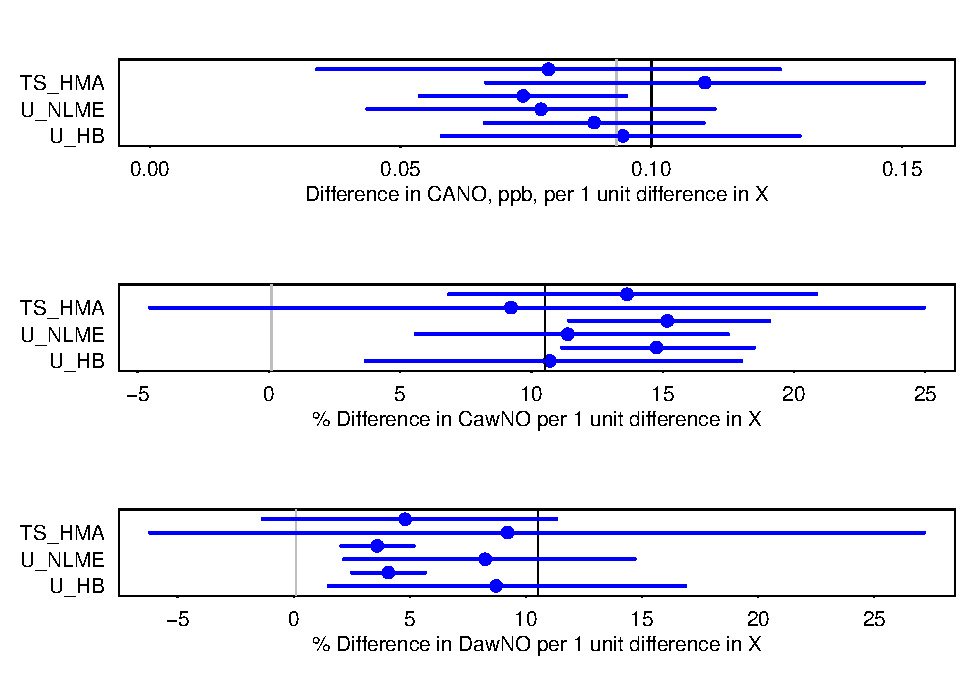
\includegraphics{DeMO_files/figure-latex/plotresults-1.pdf}

\end{document}
